\documentclass{article}
\usepackage{setspace}
\usepackage{amsmath}
\usepackage{amssymb}
\usepackage{amsthm}
\usepackage{amsfonts}
\usepackage{graphicx} 
\usepackage{float} 
\usepackage{fancyhdr}                                
\usepackage{lastpage}        
\usepackage{textcomp}                               
\usepackage{layout}   
\usepackage{subfigure} 
\usepackage{geometry}
\geometry{a4paper,scale=0.8}
\pagestyle{fancy}  
\lhead{ZHANG HUAKANG}
\chead{Assignment 3} 
\rhead{DB92760} 
\renewcommand{\baselinestretch}{1.05}
\title{Assignment 3 of CISC 1006}
\author{ZHANG HUAKANG \\ DB92760 \\ \\ Computer Science, \\Faculty of Science and Technology}
\begin{document}
    \maketitle
    \section{}
        \subsection{}
            When $0\leq y\leq 2$
            \begin{equation*}
                \begin{split}
                    f(y)=P(Y=y)=&\frac{C_3^yC_3^{2-y}}{C_6^2}
                \end{split}
            \end{equation*}
            elsewhere,
            \begin{equation*}
                \begin{split}
                    f(y)=P(Y=y)=&0
                \end{split}
            \end{equation*}
            \begin{center}
                \begin{tabular}{c| c}
                    $y$ &$f(y)=P(Y=y)$    \\
                    \hline
                    $0$&$0.2000$\\
                    $1$&$0.6000$\\
                    $2$&$0.2000$\\
                    elsewhere&$0$\\                
                \end{tabular}
            \end{center}
        \subsection{}
            \begin{itemize}
                \item $\forall y\in \mathbb{Z}$$$f(y)\geq 0$$
                \item $$\sum_{y}P(Y=y)=1$$
                \item $\forall y\in \mathbb{Z}$ $$f(y)=P(Y=y)$$
            \end{itemize}
    \section{}
        \subsection{}
            \begin{equation*}
                \begin{split}
                    P(X=x)=&\frac{C_2^{x}C_5^{3-x}}{C_7^3},(0\leq x\leq 2)
                \end{split}
            \end{equation*}
            \begin{figure}[H]
                \centering
                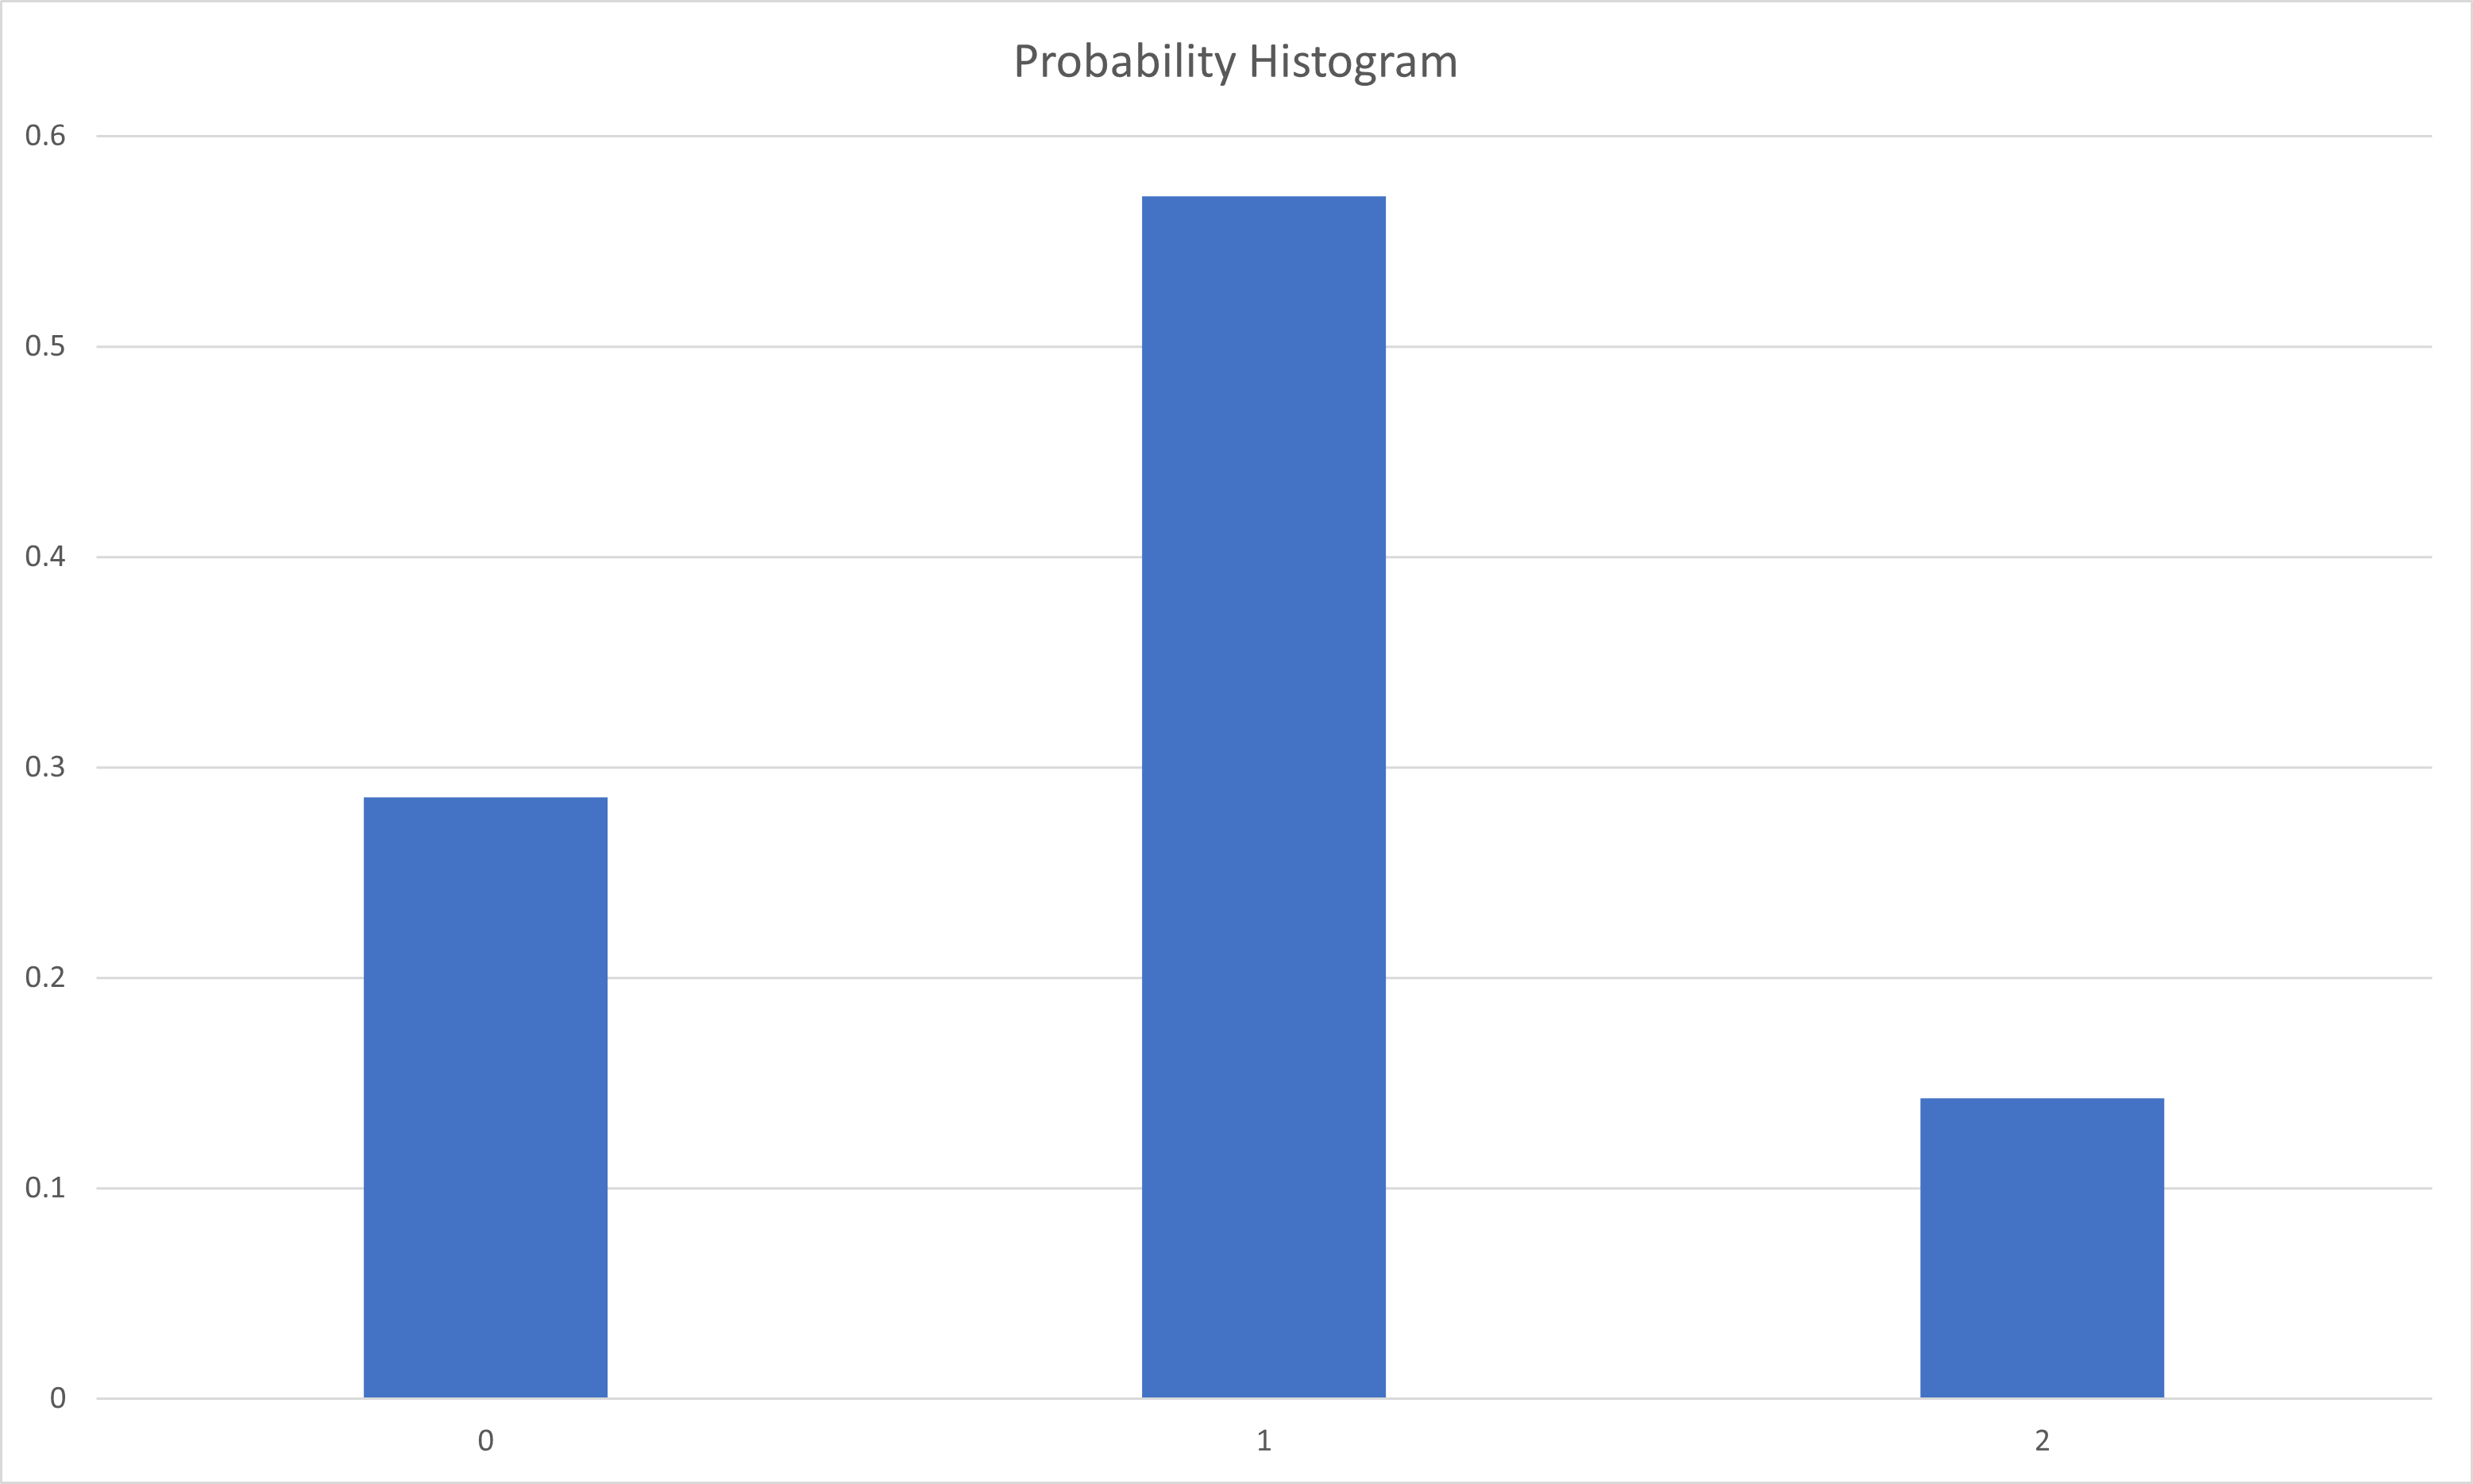
\includegraphics[width=0.9\textwidth]{img/Assignment3-01.png}
            \end{figure}
        \subsection{}
            \begin{equation*}
                \begin{split}
                    F(X=x)=&P(X\leq x)\\
                        =&\sum_{t=0}^x\frac{C_2^{t}C_5^{3-t}}{C_7^3},(0\leq x\leq 2)\\
                        &\textrm{or}\\
                        =&0,(x<0)\\
                        &\textrm{or}\\
                        =&1,(x>2)\\
                    P(X=1)=&F(X=1)-F(X=0)\\
                        \approx&0.5714\\
                    P(0<X\leq 2)=&F(X=2)-F(X=0)\\
                        \approx&0.7142\\
                \end{split}
            \end{equation*}
        \subsection{}
            \begin{figure}[H]
                \centering
                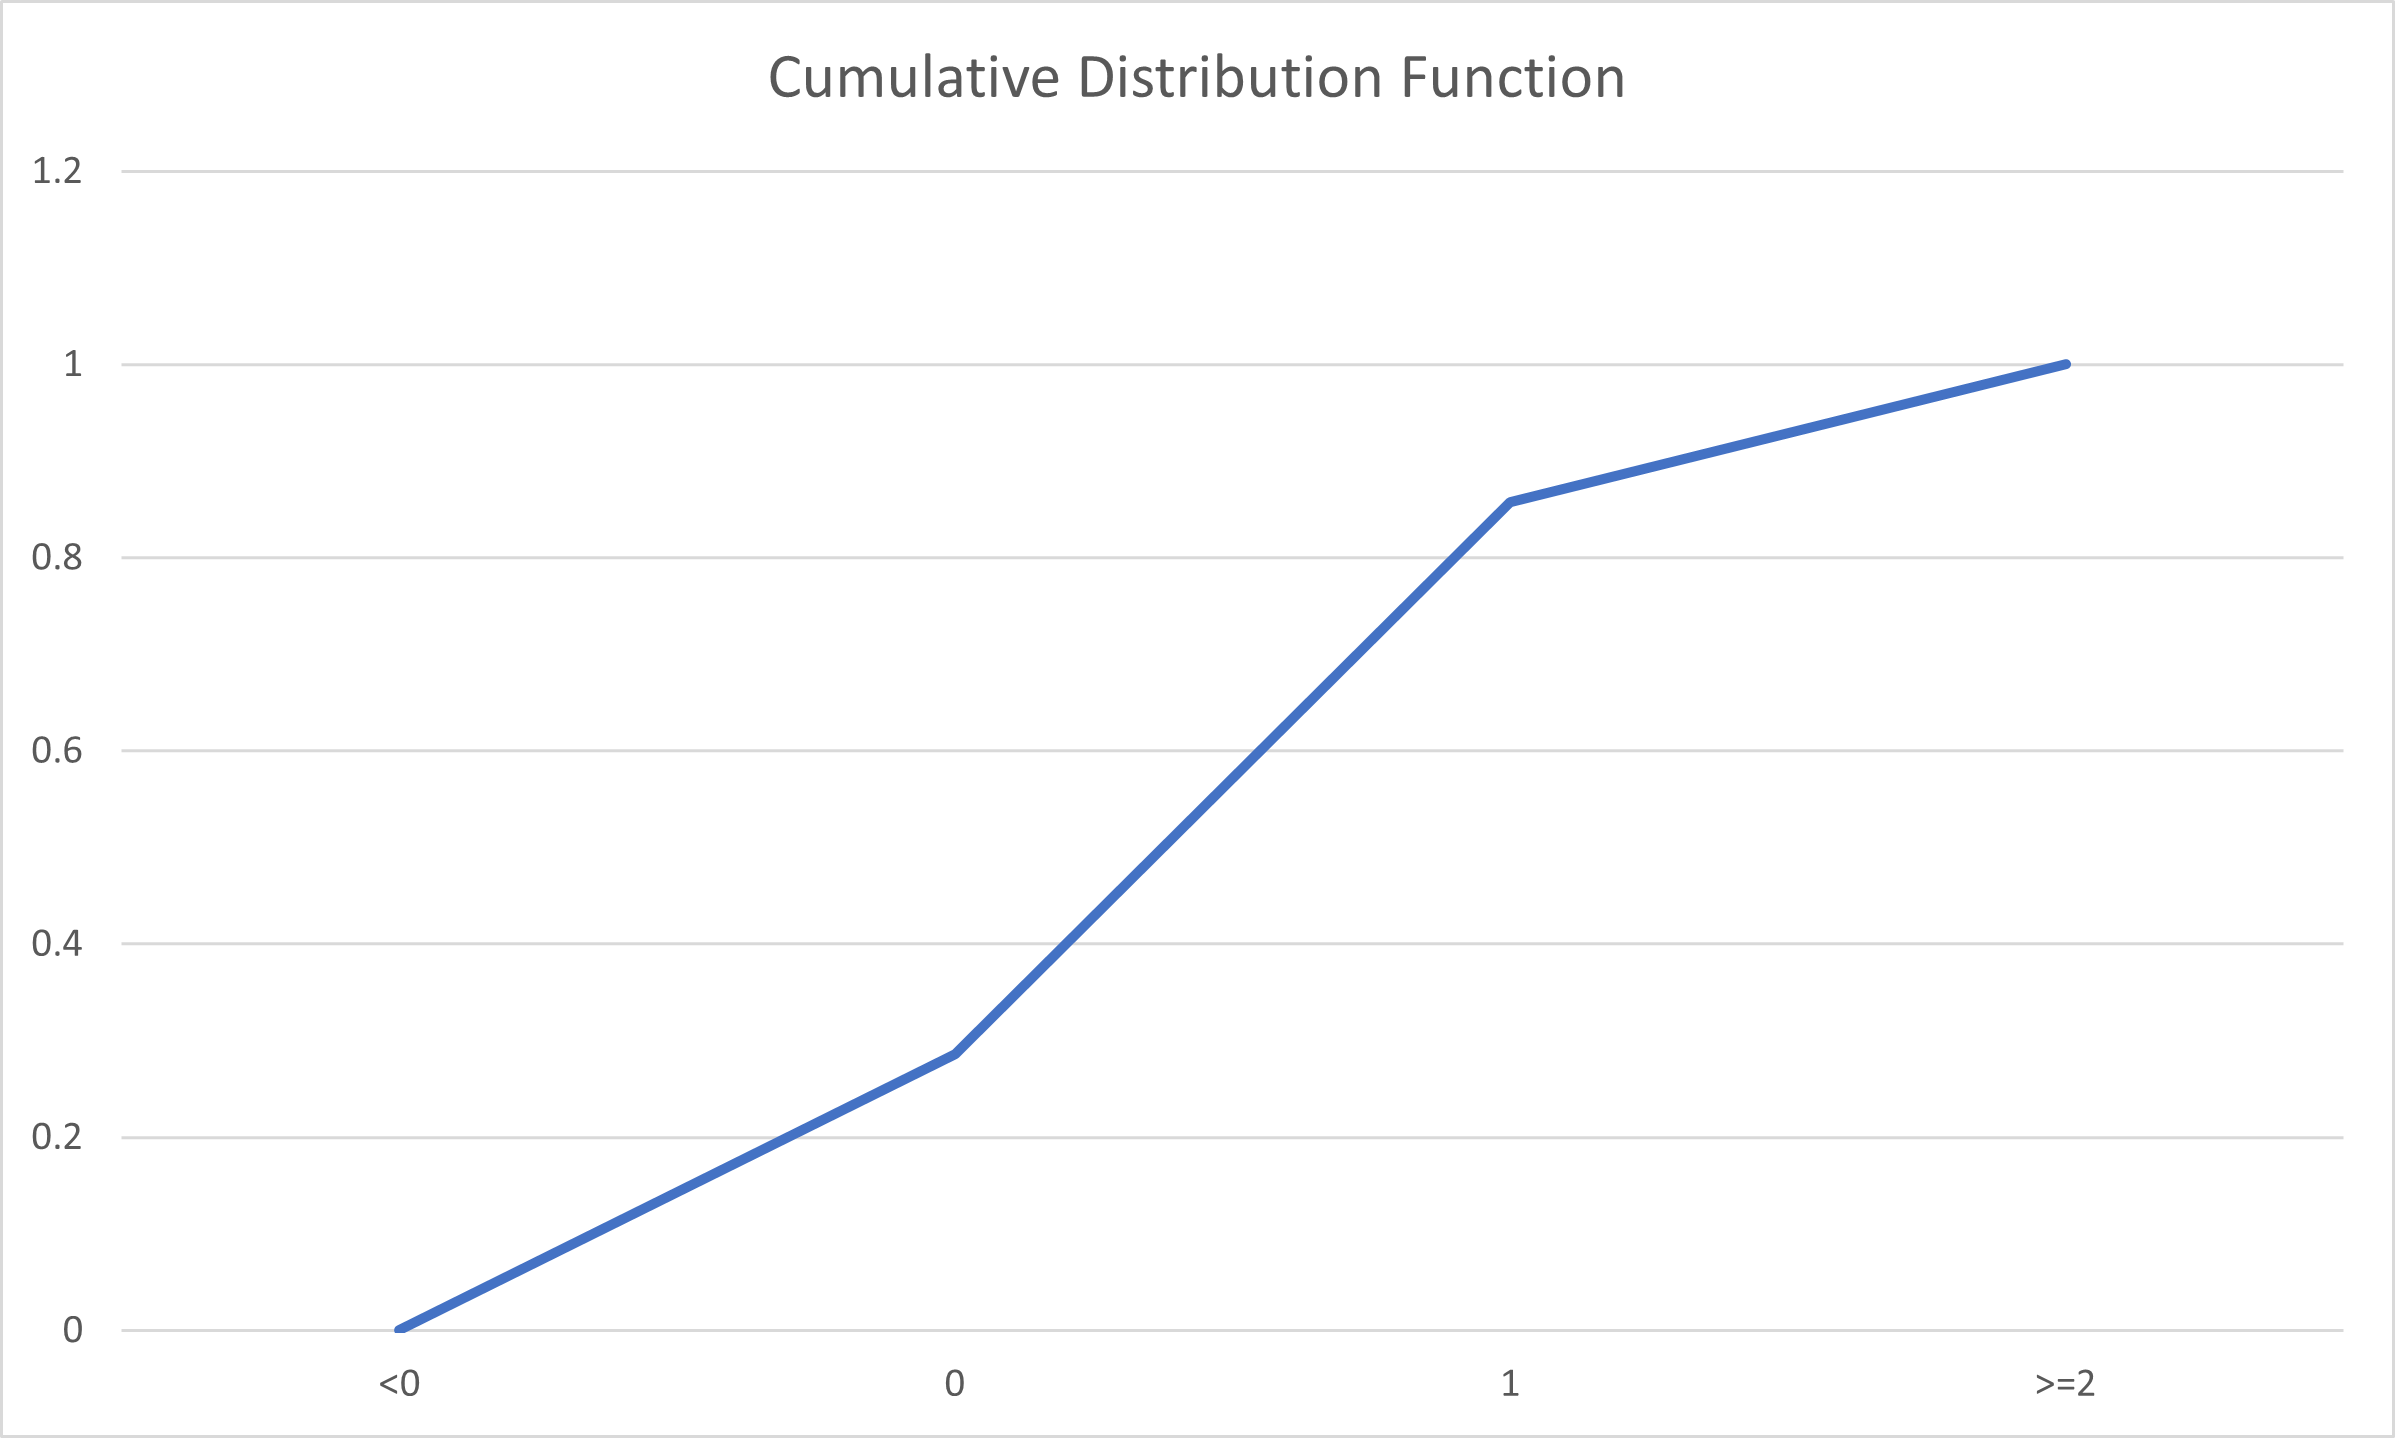
\includegraphics[width=0.9\textwidth]{img/Assignment3-02.png}
            \end{figure}
    \section{}
        \subsection{}
            \begin{equation*}
                \begin{split}
                    \int_{-\infty}^\infty f(x)dx=&\int_{-1}^1 k(2-x^2)dx+0\\
                        =&k(3x-\frac{x^3}{3})|_{-1}^1\\
                        =&2k(3-\frac{1}{3})\\
                        =&\frac{16}{3}k\\
                    \frac{16}{3}k=&1\\
                    k=&\frac{3}{16}
                \end{split}
            \end{equation*}
        \subsection{}
            \begin{equation*}
                \begin{split}
                    P(X\leq \frac{1}{2})=&\int_{-\infty}^{\frac{1}{2}}f(x)dx\\
                        =&0+\int_{-1}^\frac{1}{2} \frac{3}{16}(3-x^2)dx\\
                        =&\frac{99}{128}\\
                        \approx&0.7734
                \end{split}
            \end{equation*}
        \subsection{}
            \begin{equation*}
                \begin{split}
                    P(|X|>0.8)=&P(X<-0.8+P(X>0.8)\\
                        =&\int_{-\infty}^{-0.8}f(x)dx+\int_{0.8}^\infty f(x)dx\\
                        =&\int_{-1}^{-0.8}f(x)dx+\int_{0.8}^1 f(x)dx\\
                        =&\frac{41}{500}+\frac{41}{500}\\
                        =&\frac{41}{250}\\
                        =&0.1640
                \end{split}
            \end{equation*}
    \section{}
        \subsection{}
        
            \begin{equation*}
                \begin{split}
                    &\text{When $x\geq 0$}\\
                    F(X)=&\int_{-\infty}^{x}f(t)dt\\
                        =&\int_0^x\frac{e^{-\frac{t}{2000}}}{2000}dt\\
                        =&\int_0^x-e^{-\frac{t}{2000}}\\
                        =&1-e^{-\frac{x}{2000}}\\
                     &\text{When $x< 0$}\\
                    F(x)=&0
                \end{split}
            \end{equation*}
        \subsection{}
            \begin{equation*}
                \begin{split}
                    P(X\geq 1000)=&\int_{1000}^\infty f(x)dx\\
                        =&\lim_{t\rightarrow \infty} \int_{1000}^t \frac{e^{-\frac{t}{2000}}}{2000}dt\\
                        =&e^{-\frac{1}{2}}\\
                        \approx&0.6065\\
                \end{split}
            \end{equation*}
        \subsection{}
            \begin{equation*}
                \begin{split}
                    P(X\leq 2000)=&\int_{-\infty}^{2000} f(x)dx\\
                        =&\int_{0}^{2000} f(x)dx\\
                        =&-e^{-\frac{x}{2000}}|_0^{2000}\\
                        =&1-\frac{1}{e}\\
                        \approx&0.6321
                \end{split}
            \end{equation*}
    \section{}
        \subsection{}
            \begin{equation*}
                \begin{split}
                    \int_{-\infty}^{\infty} f(y)dy =& \int_{0}^1 f(y)dy+0\\
                        =&-(1-y)^5|_0^1\\
                        =&1-0\\
                        =&1
                \end{split}
            \end{equation*}
            $\forall y \in \mathbb{R},$
                $$f(y)\geq0$$
        \subsection{}
            \begin{equation*}
                \begin{split}
                    P(Y<10\%)=&\int_{-\infty}^{0.1}f(y)dy\\
                        =&\int_0^{0.1}f(y)dy\\
                        =&1-0.9^5+1\\
                        \approx&0.4195
                \end{split}
            \end{equation*}
        \subsection{}
            \begin{equation*}
                \begin{split}
                    P(Y>50\%)=&\int_{0.5}^{\infty}f(y)dy\\
                        =&\int_{0.5}^{1}f(y)dy\\
                        =&1-0.5^5\\
                        =&\frac{31}{32}\\
                        \approx&0.9688
                \end{split}
            \end{equation*}
\end{document}